% Copyright (c) Eclipse Arrowhead Project
%
% This program and the accompanying materials are made available under the
% terms of the Eclipse Public License 2.0 which is available at
% http://www.eclipse.org/legal/epl-2.0.
%
% SPDX-License-Identifier: EPL-2.0

\documentclass[a4paper]{arrowhead}

\usepackage[yyyymmdd]{datetime}
\usepackage{enumitem}
\usepackage{etoolbox}
\usepackage[utf8]{inputenc}
\usepackage{multirow}

\renewcommand{\dateseparator}{-}

\begin{document}

%% Arrowhead Document Properties
\ArrowheadTitle{Eclipse Arrowhead Core Documentation Reference}
\ArrowheadType{Reference Architecture}
\ArrowheadTypeShort{RA}
\ArrowheadVersion{0.1}
\ArrowheadDate{\today}
\ArrowheadAuthor{Emanuel Palm}
\ArrowheadStatus{Work in Progress}
\ArrowheadContact{emanuel.palm@pinterop.se}
\ArrowheadFooter{\href{www.arrowhead.eu}{www.arrowhead.eu}}
\ArrowheadSetup
%%

%% Front Page
\begin{center}
  \vspace*{1cm}
  \huge{\arrowtitle}

  \vspace*{0.2cm}
  \LARGE{\arrowtype}
  \vspace*{1cm}
  \vspace*{\fill}

  % \includegraphics[scale=1.5]{path/to/image}

  \vspace*{1cm}
  \vspace*{\fill}

  \begin{abstract}
    This document establishes how to read and write the documentation for entities of the \textit{Eclipse Arrowhead}, a framework designed to help create highly dynamic industrial systems.
    It also provides guidelines regarding the production of \textit{conformant} documentation, as well as describing how significant documentation can be ratified.
  \end{abstract}

  \vspace*{1cm}
\end{center}
\newpage
%%

%% Table of Contents
\tableofcontents
\newpage
%%

\section{Introduction}
\label{sec:introduction}
% Copyright (c) 2021-10-07 Eclipse Arrowhead Project
%
% This program and the accompanying materials are made available under the
% terms of the Eclipse Public License 2.0 which is available at
% http://www.eclipse.org/legal/epl-2.0.
%
% SPDX-License-Identifier: EPL-2.0

We, the Eclipse Arrowhead project, here present and authoritative set of Arrowhead concept definitions, meant to serve as the foundational language for discussions about and the modelling of Arrowhead-based designs.
The document exists to help mitigate compatibility and consistency issues in software, tooling, models and all other things of relevance to Arrowhead.
The concepts established here are not specified in terms of any particular modelling tools or languages, but should be useful as foundation for any other Arrowhead modelling or documentation effort.

The description of Arrowhead we present here should be seen as an extension of \textit{Reference Architecture Model Industrie 4.0} (RAMI4.0) \cite{adolphs2016reference}.
This means that we take key concepts from RAMI4.0 and present them here in the context of the Arrowhead framework.
As RAMI4.0 is defined partly in terms of \textit{Service-Oriented Architecture} (SOA), we also builds upon \textit{Reference Model for Service Oriented Architecture} (SOA-RM) \cite{mackenzie2006reference}.
In other words, this document assumes a world-view of service-oriented communication in an Industry 4.0 setting.
This world-view is introduced more fully in Section \ref{sec:arrowhead}.

\subsection{Primary Audiences}
\label{sec:introduction:audiences}

This document is being written and maintained with the following primary audiences in mind:

\begin{itemize}
\item \textit{System architects, integrators and developers} designing, integrating or developing Arrowhead systems.
\item \textit{Standardization engineers and researchers} seeking to extend, analyze or improve upon Arrowhead.
\item \textit{Decision makers, users and other stakeholders} that need to understand fundamental Arrowhead concepts.
\end{itemize}

Those seeking a less techincally rigorous description of Arrowhead may want to focus their reading on Section \ref{sec:arrowhead}.
Others are advised to read all sections carefully, in the order they are presented.

\subsection{Scope}
\label{sec:introduction:scope}

We understand a \textit{reference model} to be a set of definitions for technical concepts of fundamental importance to a specific problem domain.
It does not specify how its definitions should be used to design systems, either abstract or concrete.
In the context of this document, the problem domain in question must be understood to be \textit{the design of service-oriented Industry 4.0 systems}.

\GlossaryHyperRef{Reference models}{model-reference} can ve used as vocabularies for defining \GlossaryHyperRef{reference architectures}{architecture-reference}, which in turn can be used to derive \GlossaryHyperRef{concrete architectures}{architecture} and, finally, \GlossaryHyperRef{software implementations}{implementation-software}, as illustrated in Figure \ref{fig:model-implementation-hierarchy}.

\vspace*{\fill}

\begin{figure}[ht]
  \centering
  
\includegraphics{figures/model-implementation-hierarchy}
  \caption{
    The hierarchical levels comprising the steps from reference models to their software implementation, going from highly abstract to entirly concrete.
    Reference models define fundamental concepts, reference architectures adds abstracts limits to how they may be used together, concrete architectures makes those limits realizable in the real world, and implementations do realize all above levels in practice.
  }
  \label{fig:model-implementation-hierarchy}
\end{figure}

\subsection{Notational Conventions}
\label{sec:introduction:conventions}

\subsubsection{Diagrams}

A box with a name inside it denotes a named \GlossaryHyperRef{entity}{entity-model}.
A named arrow between boxes denotes the \GlossaryHyperRef{relation}{relation-model} implied by the name.
If a named arrow has an associated positive integer or range, the relation is to be considered as extending to the number of unique entities indicated by that integer or range.
A range is denoted by $x..y$, where $x$ and $y$ are positive integers and $x<y$.
Omitting $y$ when using the range notation means that the range is infinite from $x$.
A box being inside another box means that it is owned by the containing box.
See Figure \ref{fig:model-implementation-hierarchy} for an example of this graphical notation being used.

Note that this document does \textit{not} define an Arrowhead profile for SysML \cite{omg2019sysml}, or any other modelling language.
The concepts outlined here should corrsepond to the entities and relations defined by any such profiles, however.

\subsubsection{References}

Square brackets around numbers (e.g. \cite{delsing2017iot}) are references to the reference list in Section \ref{sec:references}.
The number within the brackets of any given reference corresponds to the entry with the same number in the reference list.

\subsubsection{Requirements}

Use of the words \textbf{must}, \textbf{must not}, \textbf{required}, \textbf{should}, \textbf{should not}, \textbf{recommended}, \textbf{may}, and \textbf{optional} are to be interpreted as follows when used in this document: \textbf{must} and \textbf{required} denote absolute requirements that must be adhered to for a described entity to be considered as compliant to this reference model; \textbf{must not} denotes an absolute prohibition; \textbf{should}, \textbf{should not} and \textbf{recommended} denote recommendations that should be deviated from only if special circumstances make it relevant; and, finally, \textbf{may} and \textbf{optional} denote something being truly optional.
These word definitions are derived from and are meant to capture what is outlined in RFC 2119 \cite{bradner1997keywords}.

\subsection{Relationships to Other Documents}
\label{sec:introduction:relationships}

The reference model outlined in this document is based on the following works, in order of precedence:

\begin{enumerate}
\item \textit{RAMI4.0} \cite{adolphs2016reference}, which outlines a ontological and architectural view of Industry 4.0.
As RAMI4.0 is a reference \textit{architecture} rather than a reference \textit{model}, however, its 5\textsuperscript{th} section is disregarded and its remaining sections treated as if being a reference model.
This delimitation excludes the ``architectural layers'', ``life-cycle \& value-stream'' phases and ``hierarchical levels'' of RAMI4.0.

\item \textit{SOA-RM} \cite{mackenzie2006reference}, which provides a standardized definition of SOA.
While RAMI4.0 does not include SOA-RM in its reference list, it does mention the standard and requires that all communications adhere to SOA principles. 

\item \textit{Prior work directly concerned with Arrowhead}.
This significantly includes \textit{IoT Automation: Arrowhead Framework} \cite{delsing2017iot}, which was written to provide a comprehensive overview of the framework.

\end{enumerate}

You are not assumed to have read any of the above documents prior to reading this.
Concepts derived from the above sources are reiterated in this document as necessary.

\subsection{Section Overview}
\label{sec:introduction:sections}

\begin{itemize}[leftmargin=3cm,rightmargin=0pt,labelwidth=2cm,labelsep=0pt,itemindent=0pt,parsep=0.1cm,topsep=0.1cm,align=left]

%\item[Section \ref{sec:introduction}]
%This section.

\item[Section \ref{sec:arrowhead}]
An informal overview of Arrowhead, serving both to provide a workable summary of the framework and to prepare readers for better understanding Section \ref{sec:model}.

\item[Section \ref{sec:model}]
The formal and normative description of Arrowhead.

\item[Section \ref{sec:conformance}]
A brief list of requirements, meant to help determine whether or not a given system is conforming to this document.

\item[Section \ref{sec:glossary}]
Lists all significant terms referred to or defined in this document in alphabetical order.

\item[Section \ref{sec:references}]
Lists references to publications referred to in this document.

\item[Section \ref{sec:revision}]
Records the history of changes made to this document.

\end{itemize}


\section{Overview}
\label{sec:overview}
% Copyright (c) 2021-2023 Eclipse Arrowhead Project
%
% This program and the accompanying materials are made available under the
% terms of the Eclipse Public License 2.0 which is available at
% http://www.eclipse.org/legal/epl-2.0.
%
% SPDX-License-Identifier: EPL-2.0

The \GlossaryHyperRef{framework-arrowhead}{Arrowhead framework}, which is illustrated in Figure \ref{fig:framework}, consists of two subframeworks: a \GlossaryHyperRef{framework-idea}{framework of ideas} and a \GlossaryHyperRef{framework-software}{framework of software}.
The framework of ideas formulates and frames the \GlossaryHyperRef{domain-problem}{\textit{problem domain}} the framework of software is meant to help address.
By this we mean that the framework of ideas presents the \GlossaryHyperRef{assumption}{assumptions}, \GlossaryHyperRef{concept}{concepts}, \GlossaryHyperRef{value}{values} and \GlossaryHyperRef{practice}{practices} that should be applied when \GlossaryHyperRef{specification}{specifying} \GlossaryHyperRef{architecture}{architectural} or other technical documentation and when \GlossaryHyperRef{implementation}{implementing} any kinds of Arrowhead systems or components.

\begin{figure}[ht!]
  \centering
  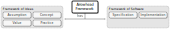
\includegraphics[scale=0.9]{figures/framework}
  \caption{
    The two subframeworks of the Arrowhead framework, concerned with \textit{ideas} and \textit{software}.
    The specifications and implementations of the software framework must conform to the assumptions, concepts, values and practices of the idea framework.
    The concepts of the idea framework are outlined in this document.
  }
  \label{fig:framework}
\end{figure}

This document is part of Arrowhead's framework of ideas.
As such, it is primarily concerned with defining concepts.
However, before we move on to consider our overview those concepts, we will first present a few examples of other key framework ideas.\footnote{
  At the time of writing, the best source of assumptions, values and practices of the Arrowhead framework is Jerker Delsing's book \textit{{IoT} Automation: Arrowhead Framework} \cite{delsing2017iot}.
  The \GlossaryHyperRef{project-eclipse-arrowhead}{Eclipse Arrowhead project} may publish other works of relevance in the future.
}
It is, for example, \textit{assumed} that the framework may be applied in contexts where the primary activity is markedly physical, such as in transportation, mining, manufacturing, electricity generation, healthcare, and so on.
One of the system characteristics \textit{valued} by the framework is \textit{resilience}, or the expectation that every system should do its outmost to mitigate and recover from degradations, failures or other contingencies that may affect its ability to perform its designated tasks.
Finally, one of its \textit{recommended practices} is that every system-of-systems should be thoroughly documented at every level, from its smallest components up to its most high-level interactions.

The rest of this section gives an overview of the most fundamental concepts of the framework.
It is meant to prepare you for the next section, where the same concepts, and other supporting concepts, are presented in greater detail.

\subsection{Stakeholders and Artifacts}

There are two kinds of members of the world of Arrowhead, (1) \GlossaryHyperRef{stakeholder}{stakeholders} and (2) \GlossaryHyperRef{artifact}{artifacts}, as depicted in Figure \ref{fig:world}.
The former denotes a \GlossaryHyperRef{person}{person} or \GlossaryHyperRef{organization}{organization} engaged in an Arrowhead enterprise, while the latter is any thing or object, tangible or intangible, that could be relevant to consider as part of such an enterprise.
Stakeholders \GlossaryHyperRef{owner}{own}, \GlossaryHyperRef{supplier}{supply}, \GlossaryHyperRef{developer}{develop}, \GlossaryHyperRef{operator}{operate}, and \GlossaryHyperRef{user}{use} artifacts, among many other possible activities.
It is their business needs and ambitions that govern what and how Arrowhead artifacts are employed.

\vfill

\begin{figure}[ht!]
  \centering
  
\includegraphics[scale=0.9]{figures/world}
  \caption{
    The two kinds of members of the Arrowhead world: stakeholders and artifacts.
  }
  \label{fig:world}
\end{figure}

\subsection{Devices, Systems and Services}

The most essential types of artifacts in the world of Arrowhead are (1) \GlossaryHyperRef{device}{hardware devices}, (2) \GlossaryHyperRef{system}{software systems} and (3) \GlossaryHyperRef{service}{services}, all shown in Figure \ref{fig:device-system-service}.
\textit{Hardware devices}, or just \textit{devices}, are physical machines, such as servers, robots or tools, that are able to maintain, or \GlossaryHyperRef{hosting-system}{\textit{host}}, \textit{software systems}.
A software system, or just \textit{system}, is a \GlossaryHyperRef{communication}{communicating} \GlossaryHyperRef{instance-software}{software instance} that \GlossaryHyperRef{provision-service}{provides} \textit{services}.
Every service represents a set of tasks a system can perform for other systems or for its stakeholders.
When a system or stakeholder makes use of a service, it is said to \GlossaryHyperRef{consumption-service}{\textit{consume}} it.

\vfill

\begin{figure}[ht!]
  \centering
  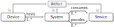
\includegraphics[scale=0.9]{figures/device-system-service}
  \caption{
    Hardware devices \textit{host} software systems, which \textit{consume} and/or \textit{provide} services.
  }
  \label{fig:device-system-service}
\end{figure}

\vfill

Every service represents one area of concern its hosting system can address.
Examples of such areas of concern could be generating financial statements, replacing propellers on drones, manufacturing bolts or measuring humidity.
A service providing control over a door could, for example, make it possible to check if the door is open, to open it and to close it.
Each such activity of every service is represented by one \GlossaryHyperRef{operation}{service operation}, which we will consider more in the next section.

\subsection{Service Provision and Consumption}

As we have already established, \GlossaryHyperRef{communication}{communication} between systems is formulated in terms of the \GlossaryHyperRef{provision-service}{provision} and \GlossaryHyperRef{consumption-service}{consumption} of \GlossaryHyperRef{service}{services}.
\GlossaryHyperRef{system}{Systems} may \textit{provide} services, which other systems can \textit{consume} by sending \GlossaryHyperRef{message}{messages} to their \GlossaryHyperRef{operation}{operations}, as depicted in Figure \ref{fig:service-consumption}.

\vfill

\begin{figure}[ht!]
  \centering
  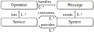
\includegraphics[scale=0.9]{figures/service-consumption}
  \caption{
    Systems consume services by sending messages to the providers of those services.
    Those providers then pass on the messages they receive to their service operations, which interpret and handle them.
  }
  \label{fig:service-consumption}
\end{figure}

\vfill

Also \GlossaryHyperRef{person}{persons} can consume services, even though it is not explicitly depicted in Figure \ref{fig:service-consumption}.
This, however, requires that a \GlossaryHyperRef{interface-human}{human interface} is attached to the providing system, or that another system with such an interface can act as \GlossaryHyperRef{proxy}{proxy}.
The human interface enables the person, via its buttons, prompts or other elements, to send messages to the services in question, just as a regular system would.

When a providing system receives a message from a consuming system or person, it passes it on to the service operation specified in that message, as described in Sections \ref{sec:concepts:service} and \ref{sec:concepts:interface}.
The operation receiving the message will then handle it by performing whatever action it describes, given that the message is \GlossaryHyperRef{message-valid}{valid} and \GlossaryHyperRef{message-permitted}{permitted}.
This handling may entail sending additional messages to other systems, starting or stopping various kinds of automation routines, reading from sensors, electronically signing contracts, sending notifications to an \GlossaryHyperRef{operator}{operator}, sending one or more messages back to the sender, among many other possible examples.

\subsection{System Composition}
\label{sec:overview:system-composition}

\GlossaryHyperRef{system}{Systems} may \GlossaryHyperRef{consumer-service}{consume services} because it is a necessary part of executing the tasks they were designed to perform.
Consider, for example, a scenario in which a number of automated guided vehicles, each of which is a system, are to move items around a factory as directed by a scheduling system.
As the scheduling system does not have wheels, engines or other necessary sensors and actuators, it cannot physically move any items by itself. 
Likewise, the individual vehicles are not capable of themselves deciding what needs to be taken to what location.
However, if the scheduling system may consume the services of the vehicles, it gains the ability to physically execute its plans.
When systems consume each others' services in this manner, they form a \GlossaryHyperRef{system-of-systems}{\textit{system-of-systems}}.

As depicted in Figure \ref{fig:systems-of-systems}, there are different kinds of systems-of-systems with their own characteristics.
There are \GlossaryHyperRef{cloud}{clouds} and \GlossaryHyperRef{system-of-clouds}{systems-of-clouds}, as well as \textit{local} and \textit{virtual} variants of both.\footnote{
  In addition to being local or virtual, a cloud may also be \textit{Arrowhead-compliant}.
  Such a cloud is referred to as an \GlossaryHyperRef{cloud-arrowhead}{\textit{Arrowhead cloud}} and conforms to various architectural requirements put forth by the \GlossaryHyperRef{project-eclipse-arrowhead}{Eclipse Arrowhead project} in a separate document.
}

\vfill

\begin{figure}[ht!]
  \centering
  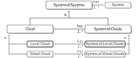
\includegraphics[scale=0.9]{figures/systems-of-systems}
  \caption{
    The types of \textit{systems-of-systems}, each of which consists of a number of \textit{systems} that consume each others' services.
    Clouds are systems-of-systems with \textit{boundaries}, while systems-of-clouds combine multiple clouds.
  }
  \label{fig:systems-of-systems}
\end{figure}

\vfill

A \textbf{cloud} is a set of systems separated from all other systems by at least one \GlossaryHyperRef{boundary-cloud}{boundary}.
Such a boundary may be formed via access control policies, firewalls, gateway systems, physical separation, among many other possible examples.
Additionally, infrastructure must be in place, of any kind, allowing for any system part of the cloud to send messages to any other system in that cloud.\footnote{
  Our term \textit{cloud} must not be confused with \textit{the cloud}, which is a common name for renting virtual compute, storage and networking resources from a so-called \textit{cloud provider}.
}

Because the Arrowhead framework is highly concerned with physical automation processes, we distinguish \GlossaryHyperRef{cloud-local}{local clouds} from \GlossaryHyperRef{cloud-virtual}{virtual clouds}.

A \textbf{local cloud} has at least one system that depends on being at a specific location to provide at least one of its services.
Examples of local clouds could be smelting stations, drone control towers, assembly lines, power distribution centers, or the components of a satellite.
All of these examples involve performing physical activities that depend on occurring at specific physical locations.
Also a common data center may be a local cloud, if its exact location matters for reasons such as privacy or performance.

On the other hand, a \textbf{virtual cloud} has no systems that depend on being at a specific location to provide their services.
In other words, all the \GlossaryHyperRef{resource}{resources} of such a cloud are \GlossaryHyperRef{virtual}{virtual}.
This is the kind of cloud that can be rented by many cloud providers and is part of the greater trend many refer to as \textit{the cloud}.
A virtual cloud could provide services for forecasting, analysis, design, planning or communication, among other possible examples.
None of these use cases require any other resources than virtual compute, storage and network resources.

Individual clouds may be interconnected to former even larger systems-of-systems, which we then refer to as \textbf{systems-of-clouds}.
The individual clouds may be owned and operated by different departments, subdivisions or teams at the same company, or even by different legal entities.
Some of them may be local, while other may be virtual.
Examples of systems-of-clouds may be a set of weather stations operated by the same company, the robots of distinct collaborating companies at a mining site, or the carriers of a supply chain.
When a system-of-clouds contain only local clouds, we refer to it as a \GlossaryHyperRef{system-of-local-clouds}{systems-of-local-clouds}.
Likewise, a system-of-clouds with only virtual clouds constitute a \GlossaryHyperRef{system-of-virtual-clouds}{systems-of-virtual-clouds}.


\section{Formats}
\label{sec:formats}
% Copyright (c) 2021 Eclipse Arrowhead Project
%
% This program and the accompanying materials are made available under the
% terms of the Eclipse Public License 2.0 which is available at
% http://www.eclipse.org/legal/epl-2.0.
%
% SPDX-License-Identifier: EPL-2.0

TODO

The three major categories of formats in which Arrowhead documentation can be expressed.
The categories are (1) print, (2) interactive, and (3) semantic.

Print documentation is concretely rendered as documents that can be printed out on paper.
Interactive documentation is presented in the form of an interactive computer application, such as a website or a plugin in a development environment.
Finally, semantic documentation exists as machine-readable definitions that can be used as input to produce other forms of documentation or generate other artifacts of interest (such as parts of computer programs).

As this document is a \textit{Reference Architecture}, it does not specify how to realize any of these three formats.
So-called \textit{Concrete Architecture} (CA) documents would have to be specified for each format of interest.
As this document is produced in LaTeX, I will write such a CA-document for LaTeX/print documentation at some later point.

\section{Framework Descriptions}
\label{sec:framework}
\input{sections/framework}

\section{Black Box Descriptions}
\label{sec:blackbox}
\input{sections/blackbox}

\section{White Box Descriptions}
\label{sec:whitebox}
% Copyright (c) 2021 Eclipse Arrowhead Project
%
% This program and the accompanying materials are made available under the
% terms of the Eclipse Public License 2.0 which is available at
% http://www.eclipse.org/legal/epl-2.0.
%
% SPDX-License-Identifier: EPL-2.0

TODO

White box descriptions (IDD, SysDD, SoSDD, SoLCDD (System-of-Local-Clouds Design Description), NetDD (Network Design Description), DevDD (Device Design Description)).

\section{Protocol Descriptions}
\label{sec:protocol}
% Copyright (c) 2021 Eclipse Arrowhead Project
%
% This program and the accompanying materials are made available under the
% terms of the Eclipse Public License 2.0 which is available at
% http://www.eclipse.org/legal/epl-2.0.
%
% SPDX-License-Identifier: EPL-2.0

TODO

Describes a complete stack of protocols on which an IDD can be formulated.
An example of a complete stack of protocols could be Ethernet, IP, TCP, and HTTP.
IP does not strictly require to be carried by Ethernet (ZigBee, WiFi and other physical protocols will do).
There should, as a consequence, be some way of indicating that any protocol below IP is acceptable.

\section{Profile Descriptions}
\label{sec:profile}
% Copyright (c) 2021 Eclipse Arrowhead Project
%
% This program and the accompanying materials are made available under the
% terms of the Eclipse Public License 2.0 which is available at
% http://www.eclipse.org/legal/epl-2.0.
%
% SPDX-License-Identifier: EPL-2.0

TODO

A profile "adds constraints" to the protocol formulated by an IDD.
A profile can define data types, header fields, prohibit certain protocol states, and so on.
An IDD referring to a profile must specify exactly what parts of the profile are applied where.

\section{Conformance Guidelines}
\label{sec:conformance}
% Copyright (c) 2021 Eclipse Arrowhead Project
%
% This program and the accompanying materials are made available under the
% terms of the Eclipse Public License 2.0 which is available at
% http://www.eclipse.org/legal/epl-2.0.
%
% SPDX-License-Identifier: EPL-2.0

TODO

A list of requirements that must be satisfied in order for a document to be considered conformant to this documentation reference.

\section{Ratification Guidelines}
\label{sec:ratification}
% Copyright (c) 2021 Eclipse Arrowhead Project
%
% This program and the accompanying materials are made available under the
% terms of the Eclipse Public License 2.0 which is available at
% http://www.eclipse.org/legal/epl-2.0.
%
% SPDX-License-Identifier: EPL-2.0

TODO

A description of the process employed by the Arrowhead project applied when ratifying or rejecting documents.
The process is to be described in such a way to allow for other organizations to reuse it.

\renewcommand{\bibsection}{\section{References}\label{sec:references}}
\bibliographystyle{arrowhead}
\bibliography{bibliography}

\newpage

\section{Revision History}
\label{sec:revision}

\subsection{Amendments}

\noindent\begin{tabularx}{\textwidth}{| p{1cm} | p{2cm} | p{1.25cm} | X | p{4cm} |} \hline
\rowcolor{gray!33} No. & Date & Version & Subject of Amendments & Author \\ \hline

1 & & & & \\ \hline

\end{tabularx}

\subsection{Quality Assurance}

\noindent\begin{tabularx}{\textwidth}{| p{1cm} | p{2cm} | p{1.25cm} | X |} \hline
\rowcolor{gray!33} No. & Date & Version & Approved by \\ \hline

1 & & & \\ \hline

\end{tabularx}

\end{document}